\documentclass{article}

\usepackage{PRIMEarxiv}

\usepackage[utf8]{inputenc}
\usepackage[T1]{fontenc}
\usepackage{url}
\usepackage{booktabs}
\usepackage{amsfonts}
\usepackage{nicefrac}
\usepackage{microtype}
\usepackage{fancyhdr}
\usepackage{graphicx}
\usepackage{subcaption}
\usepackage[hidelinks]{hyperref}
\usepackage{orcidlink}
\usepackage{amsmath}
\usepackage{tikz}
\usepackage{placeins}
\usetikzlibrary{arrows.meta, positioning, shapes.geometric, arrows, fit, backgrounds}

\graphicspath{{media/}}

\pagestyle{fancy}
\thispagestyle{empty}
\rhead{ \textit{ }}
\fancyhead[LO]{Mahlow et al. 2026}

\title{SI-FPM: A Segmented and Interpretable Facial Proportion Metric for Auditing Visual Representations
%%%% Cite as
%%%% Update your official citation here when published
%\thanks{\textit{\underline{Citation}}:
%\textbf{Authors. Title. Pages.... DOI:000000/11111.}}
}

\author{
  Felipe Mahlow \orcidlink{0000-0001-9816-1440}\\
  São Paulo State University\\
  Bauru, Brazil\\
  \texttt{f.mahlow@unesp.br} \\
  \And
  Giovanni Franco \orcidlink{0009-0002-8588-8979}\\
  São Paulo State University\\
  Bauru, Brazil\\
  \texttt{gs.franco@unesp.br}
  \And
  Guilherme Fiusa \orcidlink{0000-0002-2390-7823}\\
  University of Rochester\\
  New York, United States\\
  \texttt{gfiusa@ur.rochester.edu}
  \And
  Kelton Augusto Pontara da Costa \orcidlink{0000-0001-5458-3908}\\
  São Paulo State University\\
  Bauru, Brazil\\
  \texttt{kelton.costa@unesp.br} \\
}

\begin{document}
\maketitle

\begin{abstract}
Facial images are increasingly used in studies that require grouping, comparing, or auditing human representations. Yet, many available approaches rely either on human annotation, which can introduce subjective and socially sensitive judgments, or on opaque embeddings whose decision mechanisms are difficult to inspect. This paper introduces the Segmented and Interpretable Facial Proportion Metric (SI-FPM), a facial representation based on segmented facial regions and pairwise proportional ratios. SI-FPM converts facial segment areas into a compact vector of interpretable geometric relations, enabling scale-normalized comparison between individuals and reference groups. We further propose an explainability layer that identifies the local facial proportions that most strongly drive a proximity decision with respect to operational reference groups. The method is evaluated through identity-oriented similarity analysis, group-level auditing based on dataset-provided male/female labels, and a generated-image audit case study. We emphasize that these labels are used as operational annotations for aggregate analysis and do not represent claims about gender identity, biological sex, or individual self-identification. By combining segmentation, proportional metrics, group-level comparison, and feature-wise explanations, SI-FPM provides a transparent tool for auditing visual representations in contexts where sensitive categories must be handled with methodological and ethical care.
\end{abstract}

\keywords{Facial proportions \and Explainable AI \and Visual representation auditing \and Segmentation \and Responsible AI \and Computer Vision}


\section{Introduction}
\label{introduction}

The increasing use of facial images in computational studies has created a methodological tension. On the one hand, researchers often need to compare images, evaluate group-level patterns, or audit visual representations produced by generative systems. On the other hand, many of these analyses involve socially sensitive categories, such as gender, ethnicity, or other appearance-related group labels, where direct human labeling can introduce subjective, culturally situated, and potentially harmful judgments. Fully automated deep models may reduce manual annotation costs, but they frequently operate through high-dimensional representations that are difficult to inspect, making it unclear which visual cues support a decision.

This paper addresses that tension by proposing the Segmented and Interpretable Facial Proportion Metric (SI-FPM), a facial metric designed for transparent image comparison and representation auditing. Instead of treating facial images as opaque embeddings, SI-FPM extracts segmented facial regions and converts them into pairwise proportional ratios. The resulting vector is not intended to define human identity, gender, ethnicity, or any other social category. Rather, it provides an interpretable geometric representation that can be used to compare images against explicitly defined reference groups under a controlled experimental protocol.

The central motivation of SI-FPM is explainability. In many audit settings, the relevant question is not only whether an image is closer to one reference group than another, but also which measurable visual proportions contributed most to that proximity. For this reason, we pair the metric with a feature-wise explanation layer that ranks local proportional drivers. These drivers do not describe essential characteristics of social groups. They identify, within a dataset and a specific reference comparison, which facial ratios most reduced the distance to one operational group and increased the distance to the contrast group.

This distinction is especially important for studies involving gender- or ethnicity-related labels. Gender is fluid, multidimensional, socially mediated, and not reducible to facial appearance. Ethnicity and race are likewise historically and culturally constructed categories, not biological essences that can be inferred from facial proportions. In this work, labels such as male and female are treated only as dataset-provided operational annotations. In the text, we refer to them as Group A and Group B whenever discussing the methodological machinery, and we clarify when figures use the original dataset labels for readability. Future ethnicity-related uses of SI-FPM should be understood in the same audit-oriented sense: as analysis of representation patterns under predefined reference labels, not as classification of persons into essential categories.

The contributions of this paper are fourfold. First, we introduce SI-FPM as a segmented facial proportion metric that represents facial images through scale-normalized pairwise ratios. Second, we define a group-comparison procedure that supports both identity-oriented similarity analysis and aggregate representation auditing. Third, we propose a driver-based explanation layer that identifies the top facial ratios responsible for a group-proximity decision. Fourth, we discuss the ethical scope of the method, emphasizing its use as an audit tool rather than as a normative system for assigning sensitive identities to individuals.

The remainder of this paper is organized as follows. Section \ref{related_work} reviews work on facial measurements, segmentation-based visual analysis, bias auditing, and explainable representations. Section \ref{operational_definitions} defines the ethical and operational framing used throughout the paper. Section \ref{metric} presents the SI-FPM formulation and its group-comparison procedure. Section \ref{experiments} reports experiments on identity-oriented similarity, group-level auditing, and generated-image inspection. Section \ref{discussion} discusses ethical implications and limitations. Section \ref{conclusion} concludes the paper.


\section{Related Work}
\label{related_work}

Computational facial analysis has historically used geometric descriptors, landmarks, ratios, and anthropometric measurements to represent facial structure. Such descriptors are attractive because they expose the variables used by the model and allow researchers to inspect changes in specific facial regions. However, traditional landmark-based approaches can depend on manually defined points or detectors that may fail under occlusion, pose variation, or domain shifts. Recent segmentation models, including the Segment Anything Model (SAM) \cite{kirillov2023segment}, offer a different path by extracting region-level masks that can be converted into geometric quantities such as area, perimeter, and relative proportion.

A second relevant line of work concerns fairness and bias in automated visual systems. Prior studies have shown that models trained or evaluated on facial imagery may exhibit uneven performance across demographic groups, raising concerns about representational harms and downstream misuse \cite{buolamwini2018gender,mehrabi2021survey}. In generative AI, audits of text-to-image systems have further shown that synthetic portraits can encode stereotyped or imbalanced depictions of social categories \cite{luccioni2023stablebias}. These studies motivate methods that can quantify visual representation patterns while preserving transparency about the assumptions and labels used in the analysis.

Explainability is central to this paper. Embedding-based approaches, including CLIP-like representations \cite{clip}, can be powerful for visual comparison, but their latent dimensions are not directly interpretable as facial attributes. In contrast, SI-FPM is designed so that each feature corresponds to a named proportional relation, such as the ratio between segmented eye area and segmented face area. This makes it possible to audit not only the final proximity score, but also the specific ratios that most influenced it. The method therefore complements black-box representation learning with a structured and inspectable geometric layer.

Finally, this work follows the broader recommendation that studies involving sex- or gender-related variables must explicitly define how those variables are operationalized and avoid treating them as simple biological or visual facts \cite{heidari2016sager}. Our use of group labels is therefore intentionally restricted. The method evaluates similarity to reference groups under dataset-provided annotations; it does not infer personal identity, self-identified gender, ethnicity, or biological sex from an image.


\section{Operational Definitions and Ethical Framing}
\label{operational_definitions}

SI-FPM is proposed as an audit-oriented metric, not as a system for assigning social identity to individuals. This distinction guides the terminology used throughout the paper.

We use the term \emph{reference group} to denote a collection of images associated with a label provided by a dataset, a study protocol, or an explicitly defined audit baseline. In the experiments involving the IMDB-WIKI dataset, the available labels are male and female. For the methodological sections, we refer to these as Group A and Group B to emphasize that the algorithm operates on reference distributions, not on ontological categories. When figure labels use male/female for visual clarity, they should be read strictly as dataset annotations.

We use the term \emph{group proximity} rather than identity assignment. A test image may be closer to Group A than Group B under SI-FPM, but this means only that its segmented facial proportion vector is more similar to the reference distribution of Group A under the chosen metric. It does not imply that the depicted person belongs to that group, identifies with that group, or can be socially or biologically classified by the system.

The same restriction applies to possible future ethnicity-related applications. Ethnicity and race are complex social and historical categories whose meaning varies across countries, cultures, and institutional contexts. SI-FPM may support aggregate audits of visual representation patterns when reference labels are externally defined and ethically justified, but it should not be used to infer ethnicity or race at the individual level.

Identity-oriented experiments in this paper are treated separately. When SI-FPM is used to compare images of the same public figure, the goal is to evaluate whether facial proportion vectors retain enough stable geometric information for image-set similarity. This experiment does not support surveillance deployment or individual identification in unconstrained settings. It is included as a controlled test of representation consistency.


\section{The SI-FPM Metric}
\label{metric}

SI-FPM represents a facial image through proportional relations between segmented facial regions. Let $\mathcal{R}=\{R_1,R_2,\dots,R_n\}$ be the set of facial regions extracted from an image, where each region corresponds to a semantically defined facial component such as the face, nose, mouth, eyes, eyebrows, chin, or hair. Each region $R_i$ is represented by a polygon $P_i$ in the image plane, with vertices $\{v_{i,1},v_{i,2},\dots,v_{i,k_i}\}$.

The area of $P_i$ is computed using the standard polygon area formula:

\[
\text{Area}(P_i)=\frac{1}{2}\left|\sum_{t=1}^{k_i}x_{i,t}y_{i,t+1}-y_{i,t}x_{i,t+1}\right|,
\]

where $(x_{i,t},y_{i,t})$ are the coordinates of the $t$-th vertex and $(x_{i,k_i+1},y_{i,k_i+1})=(x_{i,1},y_{i,1})$ closes the polygon. For any pair of valid regions $(i,j)$, SI-FPM defines the facial proportion:

\[
r_{i,j}=\frac{\text{Area}(P_i)}{\text{Area}(P_j)}.
\]

The SI-FPM vector for image $x$ is the ordered collection of non-redundant pairwise ratios:

\[
\mathbf{s}(x)=[r_{1,2}, r_{1,3}, \dots, r_{i,j}, \dots, r_{n-1,n}].
\]

Because the vector is built from ratios, it is invariant to global image scaling. If all image coordinates are scaled by a factor $\alpha$, each polygon area is scaled by $\alpha^2$, and the corresponding ratio remains unchanged:

\[
r_{i,j}^{\alpha}=\frac{\alpha^2\text{Area}(P_i)}{\alpha^2\text{Area}(P_j)}=r_{i,j}.
\]

This property does not make SI-FPM invariant to all imaging conditions. Pose, expression, occlusion, segmentation quality, and perspective effects can still affect the measured regions. However, the ratio-based formulation reduces dependence on absolute image size and makes each feature directly interpretable.


\subsection{Reference Groups and Proximity Scores}
\label{score_calc}

Let $\mathcal{G}$ be a reference group containing $m$ images with SI-FPM vectors $\{\mathbf{s}_1,\mathbf{s}_2,\dots,\mathbf{s}_m\}$. A group prototype can be defined as the component-wise mean:

\[
\boldsymbol{\mu}_{\mathcal{G}}=\frac{1}{m}\sum_{k=1}^{m}\mathbf{s}_k,
\]

or, in robustness-oriented settings, as the component-wise median. For a target image $x$, group proximity can be measured through cosine similarity:

\[
C(x,\mathcal{G})=\frac{\mathbf{s}(x)\cdot\boldsymbol{\mu}_{\mathcal{G}}}{\|\mathbf{s}(x)\|\|\boldsymbol{\mu}_{\mathcal{G}}\|}.
\]

For two reference groups, $\mathcal{G}_A$ and $\mathcal{G}_B$, a target image can be assigned to the group with higher proximity:

\[
\hat{g}(x)=\arg\max_{g\in\{A,B\}} C(x,\mathcal{G}_g).
\]

This assignment should be read as a proximity decision under the chosen feature space, not as a social or biological classification. In experiments using male/female dataset labels, Group A and Group B correspond to those dataset-provided annotations.


\subsection{Feature-Level Explanation}
\label{explainability}

The main interpretability advantage of SI-FPM is that each coordinate has a semantic name. To identify which features most support a group-proximity decision, we compute a driver score for each ratio. Let $m_{g,k}$ be the median value of feature $k$ in group $g$, and let $\text{IQR}_{g,k}$ be its interquartile range. The standardized distance between a target feature $s_k(x)$ and group $g$ is:

\[
D_{g,k}(x)=\frac{|s_k(x)-m_{g,k}|}{\text{IQR}_{g,k}+\epsilon}.
\]

We weight each feature by its between-group separability:

\[
w_k=\frac{|m_{A,k}-m_{B,k}|}{\text{IQR}_{A,B,k}+\epsilon},
\]

where $\text{IQR}_{A,B,k}$ is a pooled interquartile range and $\epsilon$ avoids division by zero. The signed driver score favoring Group A over Group B is:

\[
E_k^{A\leftarrow B}(x)=w_k\left(D_{B,k}(x)-D_{A,k}(x)\right).
\]

Positive values indicate that feature $k$ brings the target image closer to Group A than to Group B; negative values indicate the reverse. The top-ranked absolute values are visualized as local drivers. These values should be interpreted as dataset- and comparison-specific evidence, not as universal traits of a social group.


\subsection{Implementation}
\label{code}

The current implementation uses LangSAM\footnote{\url{https://github.com/luca-medeiros/lang-segment-anything}}, built on SAM, to segment facial regions from text prompts. The target regions include the face, nose, mouth, eyes, eyebrows, chin, and hair when available. Left and right components can be measured separately and then aggregated when a combined region is required. If a segmentation mask is missing or unreliable, the corresponding ratio is stored as missing rather than forcing an artificial value. This prevents one failed segmentation from invalidating the full vector while preserving uncertainty in downstream analysis.


\section{Experiments}
\label{experiments}

We evaluate SI-FPM through three complementary analyses. The first tests whether facial proportion vectors preserve enough individual consistency to compare image sets of the same public figure. The second examines group-level proximity using male/female labels provided by the IMDB-WIKI dataset, treated here as Group A and Group B operational annotations. The third presents a generated-image audit layout for portraits produced by different generative AI models.


\subsection{Identity Identification}
\label{face_id}

The identity-oriented experiment evaluates representation consistency rather than deployment-ready identification. Each dataset corresponds to images of a widely recognized public figure, and the objective is to determine whether within-person SI-FPM similarity is higher than cross-person similarity.

For this initial test, we selected public figures with multiple available images: Pele, Serena Williams, Jackie Chan, Han Kang, Ayrton Senna, and Marie Curie. These examples were chosen to provide varied image sources, poses, ages, and visual contexts. SI-FPM vectors are computed for each image, and pairwise similarity is measured across image sets.

Let \(D_i\) and \(D_j\) represent two image sets associated with individuals \(i\) and \(j\). The cross-dataset similarity \(F_{i,j}\) is defined as the average cosine similarity between all valid SI-FPM vectors in the two sets:

\[
F_{i,j}=\frac{1}{|D_i||D_j|}\sum_{\mathbf{s}_a\in D_i}\sum_{\mathbf{s}_b\in D_j}\frac{\mathbf{s}_a\cdot\mathbf{s}_b}{\|\mathbf{s}_a\|\|\mathbf{s}_b\|}.
\]

The resulting matrix, shown in Figure~\ref{fig:cross-dataset-heatmap}, compares within-set and cross-set similarities. Diagonal values indicate consistency within the same public figure's image set, whereas off-diagonal values indicate similarity across different figures. This experiment is not presented as a biometric identification system. It is a controlled test of whether SI-FPM captures stable facial proportional structure across image variation.

\begin{figure}[ht]
    \centering
    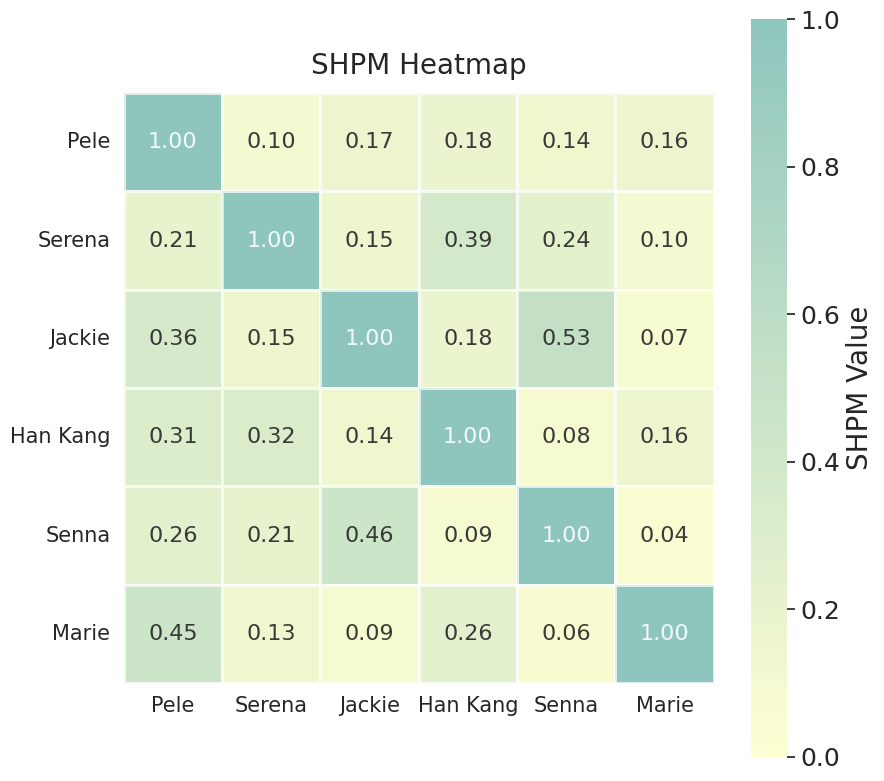
\includegraphics[width=0.7\linewidth]{shpm_cross_dataset_heatmap.png}
    \caption{Cross-dataset similarity heatmap obtained with SI-FPM. Diagonal elements represent within-set similarity for each public figure, while off-diagonal values indicate cross-set similarity.}
    \label{fig:cross-dataset-heatmap}
\end{figure}


\subsection{Group-Level Audit with Dataset Labels}
\label{gender}

The second experiment evaluates whether SI-FPM can support group-level auditing when reference labels are already present in a dataset. We use the male/female labels provided by the IMDB-WIKI dataset as operational annotations. In the methodological interpretation, these are Group A and Group B. The analysis does not attempt to infer gender identity or biological sex from images; it evaluates whether facial proportion vectors show measurable proximity patterns with respect to these existing dataset labels.

For each image, SI-FPM extracts facial ratios such as \texttt{Nose\_vs\_Face}, \texttt{Mouth\_vs\_Face}, \texttt{Eyes\_vs\_Face}, \texttt{Nose\_vs\_Mouth}, \texttt{Eyes\_vs\_Nose}, and \texttt{Eyes\_vs\_Mouth}. We then compare the distributions of these ratios between the two reference groups. Violin plots and box plots provide interpretable summaries of central tendency, dispersion, and overlap, while the t-SNE projection offers a qualitative view of the SI-FPM feature space.

The central point of this experiment is not that facial proportions determine gender. Rather, the experiment asks whether a transparent metric can reveal which proportional patterns are associated with dataset labels in aggregate. This is precisely the type of setting in which an interpretable audit method is useful: it allows researchers to inspect the variables involved in a group-level decision instead of delegating the analysis to an opaque classifier.

\begin{figure}[ht]
    \centering
    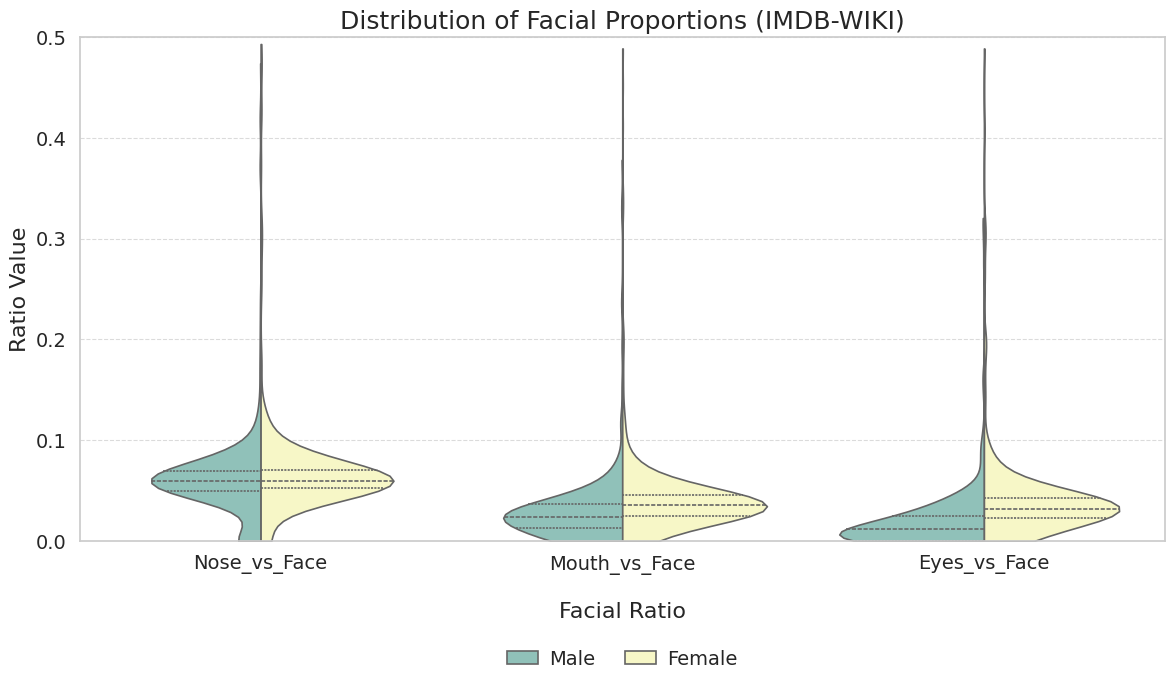
\includegraphics[width=0.85\linewidth]{violin_face_ratios_imdb_wiki.png}
    \caption{Violin plots of facial proportion distributions extracted with SI-FPM from the IMDB-WIKI dataset. The male/female labels are dataset-provided operational annotations and are interpreted in the text as Group A and Group B.}
    \label{fig:violin-face-ratios}
\end{figure}

\begin{figure}[ht]
    \centering
    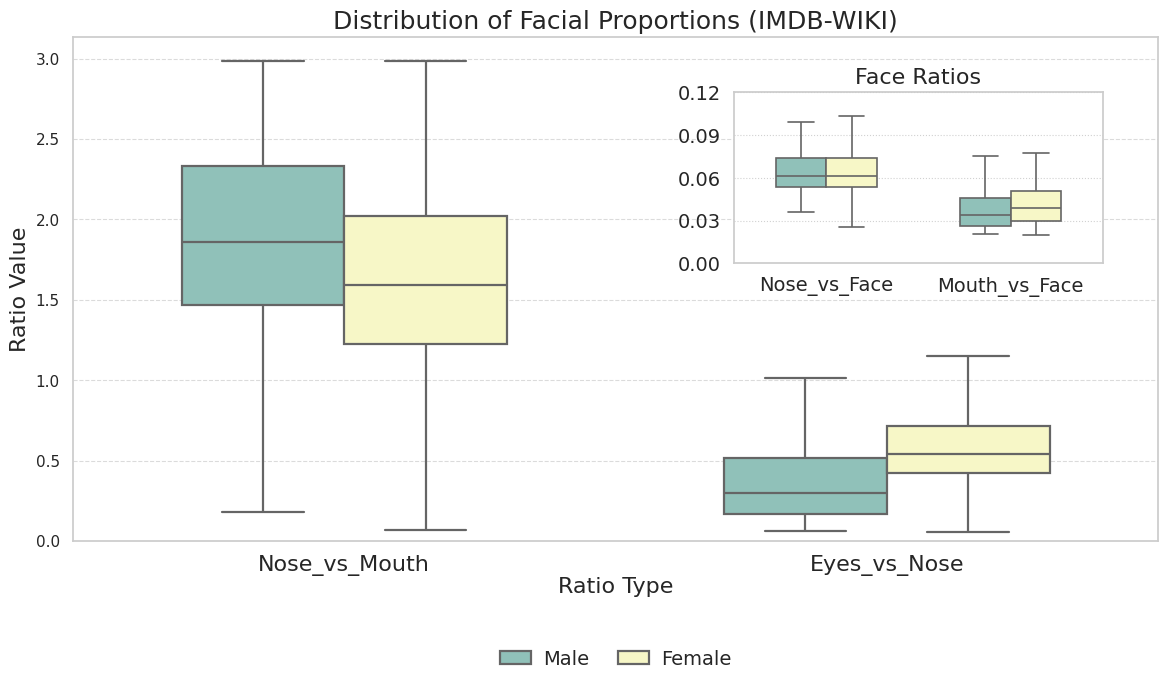
\includegraphics[width=0.9\linewidth]{boxplot_cross_ratios_imdb_wiki.png}
    \caption{Box plots of cross-facial proportions computed with SI-FPM. The plots show how specific facial ratios vary across the two dataset-provided reference groups, emphasizing distributional overlap as well as differences in central tendency.}
    \label{fig:boxplot-cross-ratios}
\end{figure}

\begin{figure}[ht]
    \centering
    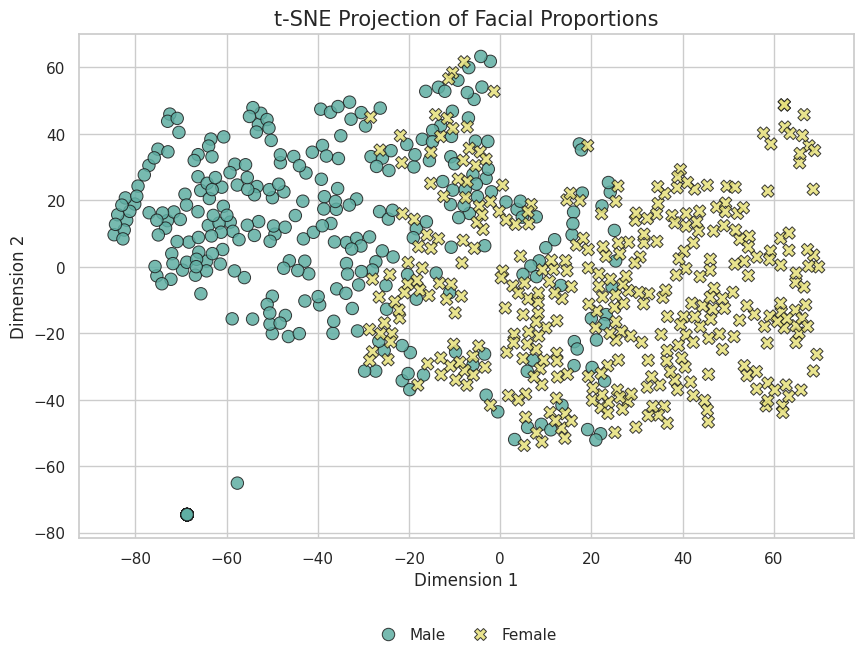
\includegraphics[width=0.85\linewidth]{tsne_facial_proportions_gender.png}
    \caption{t-SNE projection of SI-FPM vectors. Each point represents an individual image embedded in two dimensions and colored according to the dataset-provided reference label. The projection is used only as an exploratory visualization of group-level structure and overlap.}
    \label{fig:tsne-gender}
\end{figure}


\subsection{Generated-Image Audit Case Study}
\label{generated_case_study}

The final analysis is designed to audit portraits generated by different image-generation models. For each generated portrait, SI-FPM can compute its proximity to the two reference groups and display the top local drivers responsible for the decision. This format is particularly useful in AI ethics contexts because it does not merely output a category; it exposes the measurable facial ratios that contributed to the proximity score.

For each generated portrait, the audit panel combines the model output, the group-proximity scores, and the top three feature-level drivers defined in Section \ref{explainability}. This design makes the output inspectable at the level of named facial ratios, allowing the reader to evaluate which proportions contributed most to each local proximity decision.

\begin{figure}[t]
\centering

\newcommand{\Himg}{7.2cm}

\begin{minipage}{0.9\textwidth}
    \centering
    \begin{subfigure}[t]{0.42\textwidth}
        \centering
        \fbox{
\includegraphics[height=\Himg,keepaspectratio]{Flux_SHPM.png}}
        \caption{Flux}
    \end{subfigure}
    \hspace{1mm}
    \begin{subfigure}[t]{0.42\textwidth}
        \centering
        \fbox{
\includegraphics[height=\Himg,keepaspectratio]{Gemini_SHPM.png}}
        \caption{Gemini}
    \end{subfigure}
\end{minipage}

\vspace{4mm}

\begin{minipage}{0.9\textwidth}
    \centering
    \begin{subfigure}[t]{0.42\textwidth}
        \centering
        \fbox{
\includegraphics[height=\Himg,keepaspectratio]{GPT_SHPM.png}}
        \caption{GPT}
    \end{subfigure}
    \hspace{1mm}
    \begin{subfigure}[t]{0.42\textwidth}
        \centering
        \fbox{
\includegraphics[height=\Himg,keepaspectratio]{SDXL_SHPM.png}}
        \caption{SDXL}
    \end{subfigure}
\end{minipage}

% TODO before submission: replace the panel with the version computed from final SI-FPM vectors for the four generated images.
\caption{Case-level SI-FPM audit layout for portraits generated by Flux, Gemini, GPT, and SDXL. Each panel combines the generated image, group-proximity scores, and feature-level explanatory drivers.}
\label{fig:quadro-modelos}
\end{figure}

\FloatBarrier


\section{Discussion and Limitations}
\label{discussion}

SI-FPM offers a transparent alternative to purely embedding-based image comparison. Its main strength is that every feature has a direct geometric meaning, allowing researchers to inspect which proportions influence a similarity or group-proximity decision. This property is valuable for visual representation audits, where the legitimacy of the analysis depends not only on the output score but also on the ability to explain how that score was obtained.

At the same time, interpretability does not eliminate ethical risk. A transparent metric can still be misused if its outputs are framed as evidence of inherent social or biological categories. For this reason, SI-FPM should be restricted to controlled research and auditing contexts in which the reference groups, labels, datasets, and limitations are explicitly documented. In particular, results involving male/female labels should be interpreted as proximity to dataset annotations, not as inference of gender identity or biological sex.

Several technical limitations must also be considered. First, SI-FPM depends on segmentation quality. Incorrect or incomplete masks can distort area ratios, particularly for small regions such as eyes or eyebrows. Second, facial expression, pose, lighting, occlusion, image resolution, and model-generated artifacts may affect the segmented regions. Third, pairwise ratios based on areas capture only a subset of facial geometry; distances, angles, symmetry, and spatial relations may provide complementary information. Fourth, the current group-level experiments are limited to binary dataset labels. Future work should evaluate broader and more carefully documented reference structures, including cases where labels are unavailable, uncertain, or not reducible to binary categories.

Future ethnicity-related applications require additional care. Such analyses should be performed only when the research question is explicitly about aggregate representation auditing, the reference labels are ethically justified, and the results are framed as dataset- and context-specific. SI-FPM is not a method for inferring ethnicity from a face. Its appropriate role is to help researchers inspect whether visual systems produce measurable and explainable representation patterns under predefined audit conditions.


\section{Conclusion}
\label{conclusion}

This paper introduced SI-FPM, a segmented and interpretable facial proportion metric for auditing visual representations. By converting segmented facial regions into pairwise proportional ratios, SI-FPM provides a scale-normalized representation in which each feature remains human-readable. The proposed group-comparison and driver-ranking procedures allow researchers to identify not only which reference group an image is closer to under the metric, but also which facial ratios most influenced that proximity.

The method was positioned as an audit tool rather than a system for assigning sensitive identities to individuals. This framing is essential for applications involving gender- or ethnicity-related labels, where categories are socially complex and cannot be reduced to facial appearance. In the experiments, dataset-provided male/female labels are treated as operational Group A/Group B annotations, and identity-oriented analysis is used only as a controlled test of representation consistency. Overall, SI-FPM contributes a transparent and ethically bounded approach for studies that require measurable, explainable, and auditable facial representation metrics.


\section*{Acknowledgments}


\section*{Funding}
This study was funded by the Funda\c{c}\~ao de Amparo \`a Pesquisa do Estado de S\~ao Paulo (FAPESP) through Project Nos. 2024/14934-0 (F.M.) and 2025/19585-6 (G.S.F.).


\section*{Contributions}
Felipe M. and Giovanni F. conducted the experiments. Kelton P. supervised the research. Guilherme F. provided insights and strengthened the study with conceptual contributions. All authors contributed to the composition of the article and the conception of the study. The final manuscript was reviewed and approved by all authors.

\section*{Interests}
The authors declare that they have no competing interests.

\bibliographystyle{apalike-sol}
\bibliography{main}

\end{document}
